\documentclass[a4paper, 12pt]{article}
\usepackage[utf8]{inputenc}
\usepackage[T1]{fontenc}
\usepackage[french]{babel}
\usepackage{amsmath}
\usepackage{amssymb}
\usepackage{relsize}
\usepackage{mathtools}
\usepackage{algorithm}
\usepackage{graphicx}
\usepackage{listings}
\usepackage[]{algpseudocode}
\DeclarePairedDelimiter{\ceil}{\lceil}{\rceil}
\let\iff\Longleftrightarrow
\let\qed\square
\lstset{
	language=Python,
	tabsize=2
}
\newtheorem{theo}{Théorème}
\pagestyle{headings}
\title{Huffman}
\author{
\textbf{Auteurs :} Quentin Januel et Loïc Mohin \\
\textbf{Mentors :} Olivier Gipouloux et Stéphane Gaussent \\ \\
\textbf{Fait à :} Université Jean Monnet, Saint Etienne
}
\date{\today}
\begin{document}
\maketitle
\begin{abstract}
Au milieu du XXème siècle, durant sa thèse de doctorat, David Albert Huffman inventa le codage Huffman. Aujourd'hui, il est encore utilisé dans des systèmes de compression tel que JPEG, MPEG et MP3.
Dans ce rapport, on se propose d'étudier le codage d'un texte en binaire par les arbres de Huffman. En premier lieu, nous donnerons quelques définitions élémentaires, pour ensuite montrer que la rentabilité de l'algorithme est indépendante de tout choix lors de la création de l'arbre de Huffman. Nous verrons alors une utilisation concrète de ce codage, pour enfin s'intéresser à la performance et l'optimalité d'un tel codage.
\end{abstract}
\newpage
\tableofcontents{}
\newpage

\section{Prérequis}

Dans cette section, nous allons tâcher de définir les outils dont nous aurons besoin pour l'analyse des arbres de Huffman.

\subsection{Alphabet}
On appelle $\Sigma$ un alphabet dont les éléments sont appelés des lettres. \\
Un mot sur $\Sigma$ est un $n$-uplet de lettres : $m = (a_1,\ a_2,\ ...,\ a_n)$. \\
L'ensemble des mots sur $\Sigma$ est noté $\Sigma^* := \{m \in \Sigma^n,\ \forall n \in \mathbb{N}\}$. \\
Soit $m = (a_1,\ a_2,\ ...,\ a_n)$ un mot, on appelle longueur du mot $m$ notée $|m|$ l'entier $n$. \\
Enfin, on note $\varepsilon$ le mot vide (unique mot de longueur $0$). \\ \\
On peut munir $\Sigma^*$ d'une loi de composition interne, la concaténation $+$ : \\
$(a_1,\ ...,\ a_n)+(b_1,\ ...,\ b_n) = (a_1,\ ...,\ a_n,\ b_1,\ ...,\ b_n)$. \\
On observe alors que $(\Sigma^*,\ +)$ est un monoïde.

\subsection{Mot pondéré}
On dit qu'un élement $(a,\ n)\in \Sigma^*\times \mathbb{N}$ est un mot pondéré de $\Sigma$ et on notera :
\begin{enumerate}
\item $l((a,\ n)) = a$ ($l$ pour "lettre"),
\item $p((a,\ n)) = n$ ($p$ pour "poids")
\end{enumerate}
On définit alors la somme de mots pondérés $x+y = (l(x)+l(y),\ p(x)+p(y))$ et on se retrouve avec un nouveau monoïde :  $(\Sigma^*\times \mathbb{N},\ +)$.

\subsection{Arbre binaire}
Soit $E$ un ensemble, on dit que $A := (Q,\ T)$ est un arbre binaire sur $E$ avec $Q \subset E$ et $T \subset E\times \mathbb{F}_2\times E$ s'il respecte les 3 propriétés suivantes :
\begin{enumerate}
\item $\exists \ !\ r \in Q,\ \forall (x,\ b) \in Q\times \mathbb{F}_2,\ (x, b, r) \notin T$ ($r$ est appelée racine de $A$ notée $r(A)$),
\item $\forall x_2 \in Q\backslash\{r\},\ \exists \ !\ (x_1,\ b) \in Q\times \mathbb{F}_2,\ (x_1,\ b,\ x_2) \in T$, (on dit que $x_1$ est un parent de $x_2$ que l'on note $\pi(x_2)$),
\item $\forall (x_1,\ b) \in Q\times \mathbb{F}_2,\ \text{card}(\{x_2 \in Q,\ (x_1,\ b,\ x_2)\in T\}) \leq 1$.
\end{enumerate}
Les éléments de $Q$ (notés $q(A)$) sont appelés les états et les éléments de $T$ (notés $t(A)$) transitions. \\
Enfin, l'ensemble des arbres binaires sur $E$ est noté $\mathcal{A}_E$.
\newpage

\section{Arbre de Huffman}

Si l'on prend un texte quelconque et que l'on compte le nombre d'occurrences de chaque lettre afin de se retrouver avec une liste de lettres pondérées, considérées comme des arbres binaires à un état, on peut alors construire l'arbre de Huffman de ce texte en fusionnant à chaque étape les 2 arbres dont les poids des racines sont minimums jusqu'à ne se retrouver qu'avec un seul arbre. \\
Une fusion consiste à rajouter une racine telle que son fils gauche soit l'un des deux arbres et son fils gauche l'autre arbre. \\ \\
On peut ensuite encoder le texte en suivant le chemin depuis la racine jusqu'à chaque lettre en ajoutant un $0$ par transition à gauche et un $1$ pour la droite. \\
Un tel arbre n'est pas unique car on peut choisir les arbres à poids minima s'il y en a plusieurs, de plus il n'y a pas de restriction sur quel arbre mettre à gauche ou à droite au moment de fusionner. \\
L'objectif sera donc de montrer que ces choix n'affectent pas le nombre de bits nécessaires pour l'encodage.

\subsection{Définition}
Tâchons d'abord de définir quels arbres parmi les arbres binaires sont des arbres de Huffman. \\
Prenons un alphabet $\Sigma$ quelconque. Tout arbre de la forme
$$
(\{x\},\ \emptyset),\ x \in \Sigma^*\times \mathbb{N},\ |l(x)| = 1
$$
sera appelé arbre de Huffman sur $\Sigma$. \\
De plus, soient $A$ et $B$ deux arbres de Huffman et $r := r(A)+r(B)$ de telle sorte que
$$
q(A) \cap q(B) \cap \{r\} = \emptyset
$$
Alors on pose
$$
M_{A,\ B} := (q(A) \cup q(B) \cup \{r\},\ t(A)\cup t(B)\cup \{(r,\ 0,\ r(A)),\ (r,\ 1,\ r(B))\})
$$
qui est également un arbre de Huffman et on dit que $M$ est la fusion de $A$ et de $
B$. \\
Notons $\mathcal{H}_\Sigma$ l'ensemble des arbres de Huffman sur $\Sigma$. \\
On pose aussi
$$
\begin{matrix}
m: &\mathcal{H}_\Sigma\times \mathcal{H}_\Sigma &\rightarrow &\mathcal{H}_\Sigma \\
&(A,\ B) &\mapsto &M_{A,\ B}
\end{matrix}
$$

\textbf{Note :} \\
Cette partie des arbres binaires est en fait trop grande car elle prend en considération des arbres qui ne peuvent pas être amenés à être créés par l'algorithme (exemple $(\{1\},\ \{2\})$)

\subsection{Proposition 1}
Pour tout alphabet $\Sigma$, on a $\mathcal{H}_\Sigma \subset \mathcal{A}_{\Sigma^*\times \mathbb{N}}$. \\
\textbf{Preuve :} \\
Pour les arbres de Huffman de la forme $(\{x\},\ \emptyset)$ :
\begin{enumerate}
\item La racine est $x$ et est bien unique (aucune transition de la forme $(., ., x)$ vu que l'ensemble des transitions est vide).
\item Aucun état n'est pas la racine donc la propriété est trivialement vérifiée.
\item L'ensemble des transitions étant vide, le cardinal sera toujours inférieur à $1$.
\end{enumerate}
Pour les arbres de Huffman de la forme $M_{A,\ B}$ :
\begin{enumerate}
\item $r(A)$, $r(B)$ et $r$ sont les seuls candidats pour être des racines (car $A$ et $B$ sont des arbres binaires et n'ont qu'une seule racine). \\
Or on a $(r,\ 0,\ r(A))$ et $(r,\ 1,\ r(B))$ des transitions donc $r(A)$ et $r(B)$ ne sont pas racines. La racine $r$ est bien unique.
\item Soit $x$ un état n'étant pas la racine, il appartient donc soit à $q(A)$, soit à $q(B)$. S'il n'est pas racine d'un de ces sous-arbres, alors la propriété est vérifiée, sinon les transitions $(r,\ 0,\ r(A))$ et $(r,\ 1,\ r(B))$ remplissent la propriété.
\item La propriété est déjà vérifiée pour tout état qui n'est pas $r$, or seulement deux transitions sont rajoutées et on a
$$
\text{card}(\{x \in Q,\ (r,\ 0,\ x) \in T\}) = \text{card}(\{x \in Q,\ (r,\ 1,\ x) \in T\}) = 1 \leq 1
$$
\end{enumerate}
\qed

\subsection{Classification des arbres de Huffman}
L'objectif est de construire des classes d'équivalence d'arbres de Huffman selon le nombre de bits qu'ils encodent. \\
L'ensemble des feuilles d'un arbre binaire $A$ est
$$
\mathcal{F}_A := \{x_1\in q(A),\ \forall (x_1,\ b)\in q(A)\times \mathbb{F}_2,\ (x_1,\ b,\ x_2)\notin t(A)\}
$$ 
Soit $\omega$ une fonction qui à un arbre lui associe cette longueur d'encodage, on a par définition
$$
\begin{matrix}
\omega: &\mathcal{H}_\Sigma &\rightarrow &\mathbb{N} \\
&A &\mapsto &\mathlarger{\mathlarger{‎‎\sum}}_{x\in \mathcal{F}_A} n_A(x)\times p(x)‎‎
\end{matrix} \\
$$
où $n_A(x)$ est la profondeur de $x$ dans l'arbre $A$, c'est-à-dire l'entier $n$ tel que $\pi^n(x) = r(A)$. \\
On définit la relation d'équivalence
$$
A\mathcal{R}B \iff \omega(A) = \omega(B),\ \forall A,\ B \in \mathcal{H}_\Sigma
$$
On dénote également $\overline{\mathcal{H}_\Sigma} := \mathcal{H}_\Sigma/\mathcal{R}$ l'ensemble quotient de $\mathcal{H}_\Sigma$ par $\mathcal{R}$.

\subsection{Lemme}
$\forall A,\ B \in \mathcal{H}_\Sigma,\ \omega\circ m(A,\ B) = \omega(A)+p\circ r(A)+\omega(B)+p\circ r(B)$ \\
\textbf{Preuve :} \\
Soient $A$ et $B$ deux arbres de Huffman,
\begin{align*}
\omega\circ m(A,\ B) &= \sum_{x \in \mathcal{F}_{m(A,\ B)}} n_{m(A,\ B)}(x)\times p(x) \\
&= \sum_{x \in \mathcal{F}_A} (n_A(x)+1)\times p(x)+\sum_{x \in \mathcal{F}_B} (n_B(x)+1)\times p(x) \\
&= \sum_{x \in \mathcal{F}_A} n_A(x)\times p(x) + \sum_{x \in \mathcal{F}_A} p(x) + \sum_{x \in \mathcal{F}_B} n_B(x)\times p(x) + \sum_{x \in \mathcal{F}_B} p(x) \\
&= \omega(A) + p\circ r(A) + \omega(B) + p\circ r(B)
\end{align*}
\qed

\subsection{Proposition 2}
$$
\forall A \in \mathcal{H}_\Sigma,\ \omega(A) = \sum_{(x_1,\ b,\ x_2)\in t(A)} p(x_2)‎‎
$$
\textbf{Preuve :} \\
Comme chaque arbre de Huffman peut s'exprimer de la forme $m(m(...,\ ...),\ m(...,\ ...))$ jusqu'à se retrouver avec des arbres tels $(\{x\},\ \emptyset)$, procédons par récurrence sur la fonction fusion. \\
Soit $A := (\{x\},\ \emptyset)$, alors
$$
\omega(A) = 0 = \sum_{(x_1,\ b,\ x_2)\in t(A)} p(x_2)‎‎
$$
La propriété est bien vérifiée. \\
Prenons maintenant deux arbres $A$ et $B$ tels que la propriété soit vraie, vérifions la pour $m(A,\ B)$ :
\begin{align*}
\omega\circ m(A,\ B) &= \omega(A)+\omega(B)+p\circ r(A)+p\circ r(B) \\
&= \sum_{(x_1,\ b,\ x_2)\in t(A)} p(x_2)‎‎+\sum_{(x_1,\ b,\ x_2)\in t(B)} p(x_2)+\sum_{(x_1,\ b,\ x_2) \in \{(r,\ 0,\ r(A)),\ (r,\ 1,\ r(B))\}} p(x_2)‎‎ \\
&= \sum_{(x_1,\ b,\ x_2)\in t\circ m(A,\ B)} p(x_2)
\end{align*}
La propriété est donc vraie pour tout arbre de Huffman.
\qed \\

Remarque, on peut aussi démontrer que
$$
\omega(A) = \sum_{(x_1,\ b,\ x_2)\in t(A)} p(x_1)‎‎
$$

\subsection{Théorème}
Pour tout mot de $\Sigma$, l'arbre de Huffman associé est unique dans $\overline{\mathcal{H}_\Sigma}$. \\
\textbf{Preuve :} \\
Prenons un mot de $\Sigma^*$, l'algorithme de Huffman nous dit de considérer l'ensemble des arbres de Huffman de la forme$(\{(a,\ n)\},\ \emptyset)$ avec $a$ les lettres du mot et $n$ leur nombre d'occurrences. \\
Ensuite, étant donné un ensemble de $n$ arbres, il faut considérer l'ensemble de $n-1$ arbres où l'on a fusionné les deux arbres dont les poids des racines sont minimums, et ce jusqu'à ne se retrouver qu'avec un seul arbre. \\
Or ces arbres ne sont pas forcément uniques et de plus $m(A,\ B) \neq m(B,\ A)$. \\ \\
Observons ce que devient la somme des longueurs d'encodage $\omega$ d'un ensemble d'arbres $X$ après une itération de l'algorithme. \\
Soient $A$ et $B$ deux arbres de $X$ dont les poids des racines sont minimums. La nouvelle liste sera donc $Y := X\backslash\{A,\ B\}\cup\{m(A,\ B)\}$.
\begin{align*}
\sum_{C\in Y} \omega(C) &= \omega\circ m(A,\ B)+\sum_{C\in X\backslash\{A,\ B\}} \omega(C) \\
&= \omega(A)+\omega(B)+p\circ r(A)+p\circ r(B)+\sum_{C\in X\backslash\{A,\ B\}} \omega(C) \\
&= p\circ r(A)+p\circ r(B)+\sum_{C\in X} \omega(C)
\end{align*}
On constate que la somme des poids a augmenté de $p\circ r(A)+p\circ r(B)$ ce qui est indépendant de l'ordre de la fusion entre $A$ et $B$ ainsi que le choix des arbres aux poids minimums parmi tous les arbres de l'ensemble. \\ \\
Ainsi si l'algorithme a donné pour un mot $m$ deux arbres $A$ et $B$ différents, on aura quand même $\omega(A) = \omega(B) \iff A\mathcal{R}B$ ce qui montre qu'ils appartiennent à la même classe d'équivalence dans $\overline{\mathcal{H}_\Sigma}$. $\qed$ \\ \\
Profitons en pour poser $h: \Sigma^* \rightarrow \overline{\mathcal{H}_\Sigma}$ la fonction qui à un mot de $\Sigma$ y associe la classe d'équivalence dans $\overline{\mathcal{H}_\Sigma}$ des arbres de Huffman construits par l'algorithme.

\newpage

\section{Utilisation concrète}
L'intérêt même des arbres de Huffman est de compresser un message. Considérons le message $m := "caba" \in\Sigma^* := {a,\ b,\ c}$ ainsi que son arbre de Huffman associé $A:=h(m)\in\overline{\mathcal{H}_\Sigma}$. Cette section a alors pour but d'expliquer comment utiliser $A$ pour encoder $m$. \\
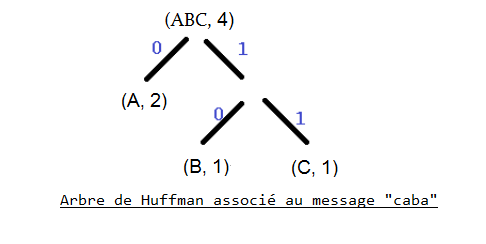
\includegraphics[width=\linewidth]{treecaba.png}

\subsection{Encodage de l'arbre lui-même}
Afin de pouvoir reconstituer le message, il faut tout d'abord trouver un moyen d'encoder l'arbre de Huffman du message en binaire. Cette tâche est simplifiée de par la définition d'arbre binaire donnée plus haut : supposons que l'arbre $A$ se note
\begin{align*}
A = (& \\
	&\{(a,\ 2),\ (b,\ 1),\ (c,\ 1),\ (bc,\ 2),\ (abc,\ 4)\}, \\
	&\{((abc,\ 4),\ 0,\ (a,\ 2)),\ ((abc,\ 4),\ 1,\ (bc,\ 2)),\ ((bc,\ 2),\ 0,\ (b,\ 1)),\ (bc,\ 2),\ 1,\ (c,\ 1))\} \\
)&
\end{align*}
On voit alors que l'arbre n'est défini que par une succession de caractères, mieux encore il peut être simplifié pour une écriture plus courte mais néanmoins toujours suffisante :
il est bon de noter que seules les transitions donnent toute l'information nécessaire de l'arbre, que les poids sont inutiles ainsi que les mots ayant une longueur supérieure à 1. De plus, la justesse de la syntaxe mathématique n'est ici pas importante. \\
Remplaçons donc chaque mot de longueur non 1 par une lettre quelconque qui n'est pas encore utilisée (ici $x$ pour $abc$ et $y$ pour $ab$). Mettons toutes les transitions gauches du côté gauche et idem pour la droite. Enfin, séparons chaque symbole par une virgule, chaque transition par 2 virgules et les deux côtés par 3 virgules. Pour l'exemple, le même arbre donnerait ceci :
$$
x,a,,y,b,,,x,y,,y,c
$$
On peut alors utiliser l'arbre en encodant chaque caractère par un nombre en binaire. Pour séparer l'arbre du début du message il est possible de rajouter à nouveau 3 virgules à la fin de l'arbre.

\textbf{Note}
Il serait aussi possible de créer l'arbre de Huffman basé sur les fréquences d'apparition des lettres de l'alphabet dans la langue française, l'avantage étant qu'il n'y aurait alors plus besoin d'encoder l'arbre pour chaque message. Seulement la compression ne sera pas optimale et suppose la langue du message.

\subsection{Encodage du message en utilisant l'arbre}
Remplaçons chaque lettre par la succession des transitions partant de la racine jusqu'à la feuille correspondante à la lettre. Une transition sera encodée par un $0$ si elle va à gauche, et par un $1$ si elle va à droite. L'algorithme de décodage ayant connaissance de l'arbre, il sait quand se termine la définition d'un caractère lorsqu'il arrive sur une feuille. \\
En utilisant l'arbre $A$ tel décrit dans ci-dessus, le message serait alors encodé par
$$
11\ 0\ 10\ 0
$$

\newpage

\section{Performance}

\subsection{Performance d'un encodage dit naïf}
Le principe d'un codage naïf est de regarder l'alphabet et de remplacer chacun de ses éléments par un nombre en binaire partant de $0$ jusqu'au dernier caractère. Par exemple si le mot est \textbf{bonneannee}, alors l'alphabet est $\{\text{b},\ \text{o},\ \text{n},\ \text{e},\ \text{a}\}$. Ici il y a $5$ caractères différents, il faut donc compter en binaire jusqu'à $4$ (car le $0$ est aussi un caractère). \\
On se retrouve avec la table de conversion suivante :
\begin{center}
	\begin{tabular}{ | c | c | c | c | c | }
		\hline
		b & o & n & e & a \\ \hline
		000 & 001 & 010 & 011 & 100 \\
		\hline
	\end{tabular}
\end{center}
Puisque le $4$ s'encode sur $3$ bits, il faudra $3$ bits par caratère et donc la longueur de l'encodage sera $3\times n$ où $n$ est la longueur du mot (ici $3\times 10 = 30$). \\
Soit $m$ un mot sur $\Sigma$, la longueur d'encodage en bits de $m$ sera donc
$$
|m|\times \ceil[\big]{\text{log}_2|\Sigma|}
$$

\subsection{Preuve de l'optimalité du codage Huffman}
A tout codage binaire, on entend par là un codage qui à un caractère associe une suite de $0$ et de $1$, on peut y associer un arbre binaire correspondant. \\
Par exemple, pour ce codage : \\
$a = 0110$ \\
$b = 01110$ \\
$c = 00$ \\
$d = 1$ \\
On peut lui associer cet arbre : \\
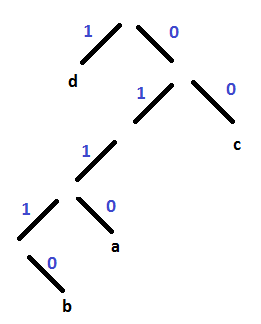
\includegraphics[width=0.3\linewidth]{tree.png}
 
Cet arbre binaire est construit de telle sorte que le nombre total en bits pour coder un message utilisant l'alphabet $\Sigma = \{a,\ b,\ c,\ d\}$ soit bien donné par : \\
$$
\omega(A) = \sum_{x\in \mathcal{F}_A} n_A(x)\times p(x)‎‎
$$

Soit $m$ un message donné, l'objectif est alors de trouver un codage tel que $\omega(A)$ soit minimal, où $A$ est l'arbre associé au codage. On dira alors qu'un tel arbre est optimal. \\

\textbf{Lemme 1 :} \\
Soit $A$ un arbre binaire, $a$ et $b$ deux feuilles de $A$. Si l'on nomme $A'$ l'arbre binaire obtenu en permutant la place de $a$ et de $b$ dans $A$, alors on obtient :
$$
\omega(A')-\omega(A) = (p(a) - p(b))\times(n_A(b) - n_A(a))
$$
\\

\textbf{Preuve :} \\
\begin{align*}
\omega(A')-\omega(A) &= \sum_{x\in \mathcal{F}_{A'}} n_{A'}(x)\times p(x)‎‎-\sum_{x\in \mathcal{F}_A} n_A(x)\times p(x)‎‎ \\
&= \sum_{x\in \mathcal{F}_A} n_{A'}(x)\times p(x)‎‎-\sum_{x\in \mathcal{F}_A} n_A(x)\times p(x)‎‎ \\
&= \sum_{x\in \mathcal{F}_A\backslash\{a,\ b\}} n_{A'}(x)\times p(x)‎‎-\sum_{x\in \mathcal{F}_A\backslash\{a,\ b\}} n_A(x)\times p(x)‎‎ \\
&+ n_{A'}(a)\times p(a) + n_{A'}(b)\times p(b) - n_A(a)\times p(a) - n_A(b)\times p(b)
\end{align*}

Or, pour tout $x \in \mathcal{F}_A\backslash\{a,\ b\}$, $n_{A'}(x) = n_A(x)$ et on a \\
$$
n_{A'}(a) = n_{A}(b),\ n_{A'}(b) = n_{A}(a)
$$

Ainsi
\begin{align*}
\omega(A')-\omega(A) &= \sum_{x\in \mathcal{F}_A\backslash\{a,\ b\}} n_A(x)\times p(x)‎‎-\sum_{x\in \mathcal{F}_A\backslash\{a,\ b\}} n_A(x)\times p(x)‎‎ \\
&+ n_A(b)\times p(a) + n_A'(a)\times p(b) - n_A(a)\times p(a) - n_A(b)\times p(b) \\
&= p(b)\times(n_A(a)-n_A(b)) + p(a)\times(n_A(b)-n_A(a)) \\
&= (p(b)+p(a))\times(n_A(b)-n_A(a))
\end{align*}
\qed \\

\textbf{Lemme 2 :} \\
Il existe un arbre optimal tel que les deux caractères avec les plus basses fréquences ont le même parent. \\

\textbf{Preuve :} \\
Soit $A$ un arbre binaire optimal, soient $a$ et $b$ les deux caractères avec la plus basse fréquence (s'il y en a plus de deux, prenons en deux au hasard dans le lot). \\
Si $a$ et $b$ ont le même parent, alors c'est bon. \\
Sinon, supposons sans perte de généralité que $n_A(a) \geq n_A(b)$. \\
Procédons alors par disjonction de cas : \\
\textbf{1.} Il existe une feuille $c$ qui a le même parent que $a$. \\
Alors soit $A'$ l'arbre binaire obtenu en inversant $c$ et $b$ dans $A$. \\
$a$ et $b$ ont alors le même parent et d'après le lemme 1
$$
\omega(A')-\omega(A) = (p(b) - p(c))\times(n_A(c) - n_A(b))
$$
Comme $a$ et $b$ sont deux caractères avec la plus basse fréquence, alors
$$
p(b)-p(c) \leq 0
$$
De plus, comme $n_A(c) = n_A(a) \geq n_A(b)$, alors $n_A(c)-n_A(b) \geq 0$. \\
Ainsi, $\omega(A')-\omega(A) \leq 0 \implies \omega(A') \leq \omega(A)$. \\
Or on avait supposé que $A$ était un arbre optimal, c'est-à-dire que pour tout autre arbre binaire $A'$, $\omega(A) \leq \omega(A')$. \\
Ainsi $\omega(A') = \omega(A)$. Donc $A'$ est également un arbre optimal. \\
\textbf{2.} $a$ est un fils unique. \\
Soit $A'$ l'arbre binaire obtenu en retirant la feuille et la branche associées à $a$ et en l'associant à son parent. \\
Alors $\omega(A') < \omega(A)$, ce qui contredit le caractère optimal de $A$. $a$ ne peut donc pas être un fils unique. \\
\textbf{3.} $a$ a le même parent qu'un sous-arbre $B$. \\
Auquel cas on peut distinguer deux sous cas : \\
\textbf{3.1.} Soit toutes les feuilles de $B$ ont une fréquence minimale. \\
On sait alors qu'il ne peut pas y avoir de feuille à fréquence minimale qui est fils unique (voir cas 2.), ce qui démontre le Lemme. \\
\textbf{3.2.} Soit il y a au moins une feuille $c$ de $B$ qui a une fréquence supérieure à la fréquence de $a$. Or si l'on pose $A'$ l'arbre où l'on a inversé $a$ et $c$ dans $A$ on se retrouve avec $\omega(A') < \omega(A)$ ce qui contredit le caractère optimal de $A$. \\
\qed

\newpage
\textbf{Théorème :} \\
Un arbre de Huffman est un arbre optimal. \\

\textbf{Preuve :}
Procédons par récurrence sur la taille du mot à coder. \\
Pour le cas $n = 1$, $\omega(A) = 0$, on ne peut pas faire mieux. \\
Soit $n > 1$ tel que tout arbre de Huffman encodant un mot de taille $n-1$ soit optimal, montrons alors que tout arbre de Huffman encodant un mot de taille $n$ est optimal aussi. \\
Soit $A$ un arbre de Huffman pour un mot $m$ de taille $n$, ainsi que $a$ et $b$ deux caractères avec la plus basse fréquence de sorte qu'ils aient le même parent $c$. \\
Considérons alors $A'$ l'arbre de Huffman de taille $n-1$, en enlevant $a$ et $b$ et en gardant $c$. \\
L'arbre $A'$ encode alors le mot $m'$, c'est-à-dire $m$ où l'on a remplacé chaque $a$ et $b$ par $c$. \\
Puisque $A'$ est un arbre de Huffman encodant un mot de taille $n-1$, il est alors optimal.
\begin{align*}
\omega(A) &= n_A(a)\times p(a) + n_A(b)\times p(b)+\sum_{x\in \mathcal{F}_A\backslash\{a,\ b\}} n_A(x)\times p(x)‎‎ \\
&= (p(a)+p(b))\times(n_A(c)+1)+\sum_{x\in \mathcal{F}_A\backslash\{a,\ b\}} n_A(x)\times p(x)‎‎ \\
&= p(c)\times(n_A(c)+1)+\sum_{x\in \mathcal{F}_{A'}\backslash\{c\}} n_{A'}(x)\times p(x)‎‎ \\
&= p(c)\times n_A(c)+p(c)+\sum_{x\in \mathcal{F}_{A'}\backslash\{c\}} n_{A'}(x)\times p(x)‎‎ \\
&= p(c)\times n_A(c)+p(a)+p(b)+\sum_{x\in \mathcal{F}_{A'}\backslash\{c\}} n_{A'}(x)\times p(x)‎‎ \\
&= p(a)+p(b)+\sum_{x\in \mathcal{F}_{A'}} n_{A'}(x)\times p(x)‎‎ \\
&= p(a)+p(b)+\omega(A')
\end{align*}

D'après le Lemme 2, il existe un arbre binaire optimal $B$ encodant $m$ tel que $a$ et $b$ aient un parent commun. \\ 
Soit $B'$ l'arbre obtenu en enlevant $a$ et $b$ de $B$. On peut alors également montrer que
$$
\omega(B) = p(a)+p(b)\omega(B')
$$
Or comme $A'$ est optimal,
\begin{align*}
\omega(B') \geq \omega(A') &\implies p(a)+p(b)+\omega(B') >= p(a)+p(b)+\omega(A') \\
&\implies \omega(B) \geq \omega(A)
\end{align*}
Ce qui montre que $A$ est un arbre optimal. \qed \\

Ainsi, le codage Huffman est le plus optimal qui soit.

\newpage

\section{Ouverture}

\subsection{Combinatoire}
On s'intéresse à compter le nombre d'arbres binaires complets à $n$ feuilles. \\
On considère que deux arbres sont les mêmes si l'on peut obtenir l'un en inversant le sous-arbre droit avec le sous-arbre gauche dans des noeuds donnés. \\
Pour $n = 1$, il existe un unique arbre. Pour $n = 2$ et $n = 3$, idem. Le cas de $n = 3$ est un peu plus subtil car l'on pourrait croire qu'il existe deux arbres différents mais une simple permutation des sous-arbres au niveau de la racine suffit à retrouver l'autre arbre. \\
En continuant ainsi, on obtient la suite suivante : \\
$$
1, 1, 1, 2, 3, 6, 11, 24, 47, 103, ...
$$
Il est possible de définir cette suite par récurrence. \\
En effet, pour $n$ entier, un arbre à $n$ feuilles est forcément la fusion de deux arbres à $p$ et $q$ feuilles tel que $p+q = n$. \\
Il s'agit donc la fusion de deux arbres à $p$ et $n-p$ feuilles avec $p$ inférieur ou égal à $n$.
Il faut donc sommer de $p$ entier jusqu'à $n$ le nombre d'arbres à $p$ feuilles multiplié par le nombre d'arbres à $n-p$ feuilles.
Cela nous donne la formule suivante :
$$
u_n = \sum_{p = 1}^{\ceil[\big]{n/2}} u_p\times u_{n-p},\ \forall n \in \mathbb{N}^*
$$
\\
Après une rapide recherche dans l'OEIS, il se trouve que cette suite porte le nom de \textbf{half Catalan numbers} (ou \textbf{demi nombres de Catalan}), on voit aisément d'où vient le nom car les nombres de Catalan sont générés à partir de la même formule à l'exception que la somme va jusqu'à $n$. Malheureusement il n'existe pas de formule non récursive des demi nombres de Catalan.

\subsection{Complexité de Kolmogorov}
La complexité de Kolmogorov $K$ permet de quantifier le nombre de caractères nécessaires minimum afin de produire une chaine de texte dans un langage de programmation donné. \\
C'est-à-dire que, si l'on considère le langage Python par exemple, alors $K(\text{texte}) = 10$ signifierait que le nombre minimum de caractères Python pour afficher \textbf{texte} est $10$.
Le choix du langage n'a pas d'importance.
Exemple : \\
\textbf{print("Hello world")} permet d'afficher le texte \textbf{Hello world}, on a donc
$$
K(\text{Hello world}) \leq 20
$$
Il est très facile de montrer que pour tout langage, il existe une constante $p$ telle que pour tout texte $t$, on a $K(t) \leq |t|+p$. \\ \\
On peut utiliser cette complexité afin de déterminer l'optimalité de compression d'une chaine de caractères donnée, cependant cela ne correspond pas à un codage par symbole, ne remettant alors pas en cause l'optimalité de Huffman dans son domaine. \\ \\
Fâcheusement, il est impossible de construire une fonction calculant la complexité de Kolmogorov, même si on pourrait croire que construire un tel algorithme est possible au premier abord naïf : \\

\begin{algorithm}
\begin{algorithmic}[1]
\Function{KolmogorovComplexity}{s}
\For{$i = n \textbf{ to } \infty$}
\For{$\textbf{each string p of length exactly } n$}
\If{$\textbf{isValidProgram}(p) \textbf{ and } \textbf{evaluate}(p) = s$}
\State \Return $n$
\EndIf
\EndFor
\EndFor
\EndFunction
\end{algorithmic}
\end{algorithm}

Le principe étant de générer toutes les chaines de texte à $n$ caractères en incrémentant $n$ petit à petit jusqu'à tomber sur un code qui générera le texte demandé. \\
Cependant un tel algorithme ne peut pas marcher à cause de la fonction \textbf{isValidProgram}. En effet, même s'il est possible de vérifier si un code contient ou non des erreurs de syntaxe, il est en revanche impossible de savoir si le programme ne se retrouvera pas coincé dans une boucle infinie (voir \textbf{halting problem} pour plus d'informations, la preuve consiste à supposer qu'il est possible de détecter les boucles infinies pour ensuite arriver à une contradiction). \\

Prouvons maintenant que n'importe quel programme échouerait à la tâche de calculer la complexité de Kolmogorov d'un texte donné par l'absurde ; supposons d'abord qu'on a un tel programme et qu'il fait $X$ caractères. On peut alors écrire le code suivant à la suite de notre programme : \\

\begin{algorithm}
\begin{algorithmic}[1]
\Function{KolmogorovComplexity}{}
\For{$i = n \textbf{ to } \infty$}
\For{$\textbf{each string s of length exactly } n$}
\If{$\textbf{KolmogorovComplexity}(s) > X+1000$}
\State \Return $s$
\EndIf
\EndFor
\EndFor
\EndFunction
\end{algorithmic}
\end{algorithm}
\newpage
Le programme est supposé générer des chaines de caractères de plus en plus longues jusqu'à ce qu'une ait une complexité supérieure à $X+1000$, ce qui existe puisque la complexité de Kolmogorov peut être arbitrairement grande. Cependant, ce programme comporte moins de $X+1000$ caractères et est donc une contradiction. \\
Moins formellement, ce paradoxe utilise la même contradiction que le paradoxe de Berry : "Le plus petit entier qui ne peut pas être défini en moins de 20 mots".

% \subsection{Entropie}

% Mets ici si tu veux parler de l'entropie

\newpage

\section{Conclusion}

Nous souhaiterions d'abord remercier M. Gaussent et M. Gipouloux de nous avoir introduit aux arbres de Huffman ainsi que pour leur encadrement. \\

Lors de ce problème ouvert, nous avons pu aboutir à quelques résultats, certains essentiels comme l'équivalence des arbres de Huffman et leurs optimalités, et d'autres moins importants. \\
Certaines pistes n'ont malheureusement pas abouti, mais ce fut tout de même passionant de travailler dessus. \\

Pour finir, notons que nous aurions également pu traiter de l'entropie, d'autres méthodes de construction d'arbres de Huffman, ou d'autres codages qui ne sont pas des codages par symbole, à l'instar du codage arithmétique.

\newpage

\section{Annexes}
\subsection{Preuve spécifique que le codage Huffman est meilleur que le naïf}
Cette partie est une preuve que, dans un cas particulier, le codage Huffman est meilleur. On s'est attelé à la démontrer avant de montrer que le codage Huffman était de toute façon optimal dans tous les cas. \\

Considérons tout d'abord un mot $m$ tel que son arbre de Huffman associé soit de profondeur maximum pour un minimum de caractères différents. C'est dans ce cas précis que nous allons essayer de montrer que le codage Huffman est plus efficace. \\
Pour ce faire, considérons un arbre à $2$ feuilles de poids $1$. La racine vaudra donc $2$. Il est possible de fusionner cet arbre avec un arbre à $1$ feuille de poids $1$ et notre nouvel arbre aura désormais une racine de poids $3$. Cependant maintenant il est impossible de fusionner cet arbre avec un arbre de poids inférieur à $2$ sinon il aurait d'abord fallu associer cet arbre avec l'arbre à $1$ feuille de poids $1$. \\
En procédant ainsi jusqu'à obtenir un arbre $A$ à $n$ feuilles on obtient un arbre de profondeur maximale tout en minimisant l'écart entre les poids au fur et à mesure de la construction de l'arbre. \\ \\
On constate alors que les poids des feuilles suivent la suite de Fibonacci et on a
\begin{align*}
\omega(A) &= \sum_{(x_1,\ b,\ x_2)\in t(A)} p(x_2)‎‎ \\
&= \sum_{i = 0}^{n-2} \text{Fibo}(i)+\text{Fibo}(i+1) \\
&= \sum_{i = 0}^{n-2} \text{Fibo}(i+2) = \sum_{i = 2}^n \text{Fibo}(i)
\end{align*}
où $\text{Fibo}(n)$ est le $n$-ième nombre de Fibonacci et $n = |\Sigma|$. \\
Quant à la longueur d'encodage si le codage naïf avait été utilisé à la place, on a
$$
(1+\sum_{i = 0}^{n-2}\text{Fibo}(i))\times \ceil[\big]{\text{log}_2(n)}
$$

Prouvons par réccurence sur $n$ que l'on a toujours
$$
\sum_{i = 2}^n \text{Fibo}(i) \leq (1+\sum_{i = 0}^{n-2}\text{Fibo}(i))\times \ceil[\big]{\text{log}_2(n)}
$$
On a vérifié à l'aide de Python que la proposition est vraie jusqu'au rang $n = 5$, supposons maintenant que la propriété est vraie jusqu'au rang $n$ et vérifions si elle est vraie au rang $n+1$. \\
Déjà, puisque la suite $\frac{\text{Fibo}(n)}{\text{Fibo}(n-1)}$ tend vers $\phi < 2$ et est croissante, alors
$$
\frac{\text{Fibo}(n)}{\text{Fibo}(n-1)}+1 \leq 3\ \forall n \in \mathbb{N*}
$$
De plus
$$
\forall n > 4,\ \ceil[\big]{\text{log}_2(n)} \geq 3
$$
On peut donc partir de l'inégalité
\begin{align*}
&\ \frac{\text{Fibo}(n)}{\text{Fibo}(n-1)}+1 \leq \ceil[\big]{\text{log}_2(n)} \\
\implies&\ \text{Fibo}(n-1)\times(\frac{\text{Fibo}(n)}{\text{Fibo}(n-1)}+1) \leq \text{Fibo}(n-1)\times\ceil[\big]{\text{log}_2(n)} \\
\implies&\ \text{Fibo}(n)+\text{Fibo}(n-1) \leq \text{Fibo}(n-1)\times\ceil[\big]{\text{log}_2(n)} \\
\implies&\ \text{Fibo}(n+1) \leq \text{Fibo}(n-1)\times\ceil[\big]{\text{log}_2(n)} \\
\implies&\ \text{Fibo}(n+1) \leq \text{Fibo}(n-1)\times\ceil[\big]{\text{log}_2(n)} \\
\implies&\ B := \text{Fibo}(n+1)+(1+\sum_{i = 0}^{n-2}\text{Fibo}(i))\times \ceil[\big]{\text{log}_2(n)} \\
&\leq (1+\text{Fibo}(n-1)+\sum_{i = 0}^{n-2}\text{Fibo}(i))\times \ceil[\big]{\text{log}_2(n)} =: C
\end{align*}
Or on a
\begin{align*}
C &= (1+\sum_{i = 0}^{n-1}\text{Fibo}(i))\times \ceil[\big]{\text{log}_2(n)} \\
&\leq (1+\sum_{i = 0}^{n-1}\text{Fibo}(i))\times \ceil[\big]{\text{log}_2(n+1)} =: D
\end{align*}
Enfin, d'après l'hypothèse de réccurence on a
\begin{align*}
A :=&\ \sum_{i = 2}^{n+1} \text{Fibo}(i) \\
=&\ \text{Fibo}(n+1)+\sum_{i = 2}^n \text{Fibo}(i) \\
\leq&\ \text{Fibo}(n+1)+(1+\sum_{i = 0}^{n-2}\text{Fibo}(i))\times \ceil[\big]{\text{log}_2(n)} = B
\end{align*}
Au final on constate que $A \leq B \leq C \leq D \implies A \leq D$ \\
\qed

\subsection{Code Python}
Nous avions commencé par codé un script Python qui encodait un texte en binaire en utilisant le codage Huffman. \\
\lstinputlisting{huffman.py}

\end{document}
